% begin module limits-infinite-ex8
\begin{frame}
\frametitle{Infinite Limits}
\begin{example}[Example 8, p. 101]
Find $\lim_{x\rightarrow 0} \frac{1}{x^2}$ if it exists.
\begin{columns}[c]
\column{.6\textwidth}
\ 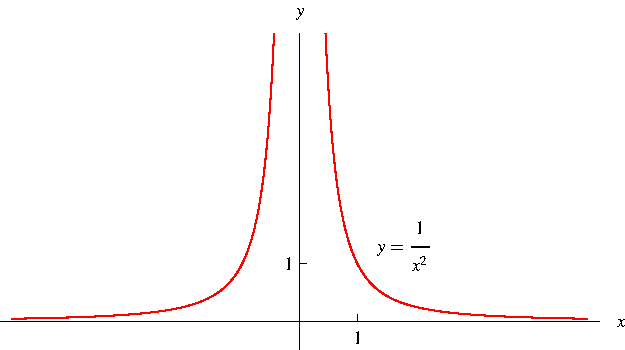
\includegraphics[height=3.7cm]{limits/pictures/02-02-xminustwo.pdf}%
\column{.4\textwidth}
\uncover<2->{
\belowdisplayskip=0pt
\[
\begin{array}{|r@{.}l|r|}
\hline
\multicolumn{2}{|c|}{x} &
\multicolumn{1}{|c|}{\frac{1}{x^2}} \\
\hline
\multicolumn{2}{|l|}{\pm 1}  %
& 1 \\
\pm 0 & 5 %
& 4 \\
\pm 0 & 2 %
& 25 \\
\pm 0 & 1 %
& 100 \\
\pm 0 & 05 %
& 400 \\
\pm 0 & 01 %
& 10,000 \\
\pm 0 & 001 %
& 1,000,000 \\
\hline
\end{array}
\]
}
\end{columns}
\begin{itemize}
\item<2->  As $x$ gets close to 0, so does $x^2$,  so $1/x^2$ gets large. 
\item<3->  $1/x^2$ can be made arbitrarily large by taking $x$ close enough to 0.
\item<4->  $f(x)$ doesn't approach a number, so $\lim_{x\rightarrow 0} 1/x^2$ doesn't exist.
\end{itemize}
\end{example}
\end{frame}
% end module limits-infinite-ex8
